\documentclass[nochap, headernames]{config/ejercicios}

\title{Prácticas Filogenia molecular (PHYLO)}
\author{Sandra Mingo Ramírez}
\date{2024/25}

\usepackage[all]{nowidow}
\usepackage{listing}
\usepackage{color}
\usepackage{tabularx}
\usepackage{multirow}
\usepackage{makecell}
\usepackage{amsmath}
\usepackage{array}
\usepackage{hyperref}

\begin{document}

\maketitle

%Programas adicionales: Genius, Ugene (alternativa gratuita de genius), Phylemon
%SeaView es un programa muy simple que permite arrastrar cualquier archivo para abrir alineamientos o árboles. Permite realizar funciones simples, pero que podrían ser laboriosas en otros programas, como por ejemplo eliminar el nucleótido en la posición X. 

\section{Formatos de archivos  filogenéticos y alineamientos}
El objetivo es familiarizarse con la conversión de formatos de archivo, diferentes métodos de alineación, eliminación de posiciones ambiguamente alineadas, edición de matrices y traducción de secuencias de ADN a proteínas.
\begin{enumerate}
\item Alinea el conjunto de datos utilizando MAFFT (en línea) con la estrategia Auto. Guarda el alineamiento resultante en formato fasta. \footnote{Los archivos fasta empiezan con el símbolo > seguido de un descriptor de la secuencia. Después, empieza la secuencia en una nueva línea. Cuando termine, hay un nuevo prompt con un nuevo descriptor.}
\item Alinea el conjunto de datos utilizando CDS-ProtAl: Utilidades > Utilidades de Alineación > CDS-ProtAl > Examinar servidor > Cargar nuevo archivo, Seleccionar formato > Secuencias no alineadas > Cargar > Aceptar, Parámetros > Mantener huecos, Código genético > Estándar. Ejecutar.
\item Compara las dos alineaciones resultantes utilizando SeaView. Arrastra el archivo de salida MAFFT. Luego Archivo > Nueva Ventana, arrastre el archivo de salida CDS-ProtAl.
\item Utiliza TrimAl para eliminar las posiciones ambiguamente alineadas. Esto puede hacerse automáticamente (redirigiendo el archivo resultante de CDS-ProtAl en Phylemon) o manualmente (Utilidades > Utilidades de Alineación > TrimAl). Selecciona Método 'sin huecos' para este ejercicio.
\item Utiliza SeaView para traducir una matriz de secuencia de nucleótidos a aminoácidos. Utiliza el conjunto de datos de TrimAl. Arrastra el archivo. Props > Ver como proteínas. Archivo > Guardar prot alineación. \textbf{Nota}: Si es necesario, se puede cambiar el código genético: Edit > Set genetic code.
\item Familiarízate con la conversión de formatos de archivo utilizando ALTER. Introduce el archivo de entrada en formato fasta (paneles de la izquierda): 
\begin{enumerate}
\item Seleccionar formato > Autodetectar
\item Cargar o pegar MSA > Seleccionar sistema operativo > Linux / Mac OS X. Seleccione el de salida (paneles derechos): Seleccionar programa > RAxML, formato > PHYLIP, Convertir
\item Guardar MSA convertido > Seleccionar sistema operativo > Linux / Mac OS X, Guardar
\item Repita la exportación al formato Nexus (Seleccione programa > MrBayes, formato > NEXUS).
\end{enumerate}
\end{enumerate}

MAFFT es un programa muy utilizado. Tiene una versión descargable y una versión en línea que permite utilizar los servidores localizados en Japón. La versión en línea cuenta con un cuadro donde pegar los datos, aunque también se puede seleccionar un archivo desde el disco duro. En nuestro caso, subiremos el archivo \texttt{HRSV-A\_modif\_RAW.fas}. Se pueden elegir algunas opciones de estética, como el uso de mayúsculas y minúsculas (la convención es poner los nucleótidos en minúscula y los aminoácidos en mayúscula), la dirección de las secuencias (se le puede pedir al programa que compruebe y ajuste la direccionalidad, aunque consume más recursos y tarda más tiempo) y el orden de la salida. Poner un nombre al trabajo puede ser útil cuando se van a lanzar varios trabajos simultáneamente. También permite poner una dirección de correo que notifique cuando se ha terminado de analizar un trabajo que vaya a tardar mucho para evitar tener que estar con la pestaña del ordenador abierta. Entre la configuración avanzada, se puede seleccionar la estrategia. Los métodos progresivos van alineando las secuencias en parejas y las van alineando poco a poco, añadiendo gaps donde toque según ese alinamiento. Los métodos iterativos, después de alinear todas las secuencias, vuelve al principio a reevaluar el alineamiento y mejorándolo. Por este motivo, los métodos iterativos son más lentos y se recomiendan para sets de pocas secuencias. También hay una estrategia automática que evalúa cuatro de los algoritmos según el tamaño de los datos y utiliza uno u otro. El resultado del alineamiento después de darle al botón de Submit es el que aparece en la imagen \ref{fig:mafft-result}.

\begin{figure}
\centering
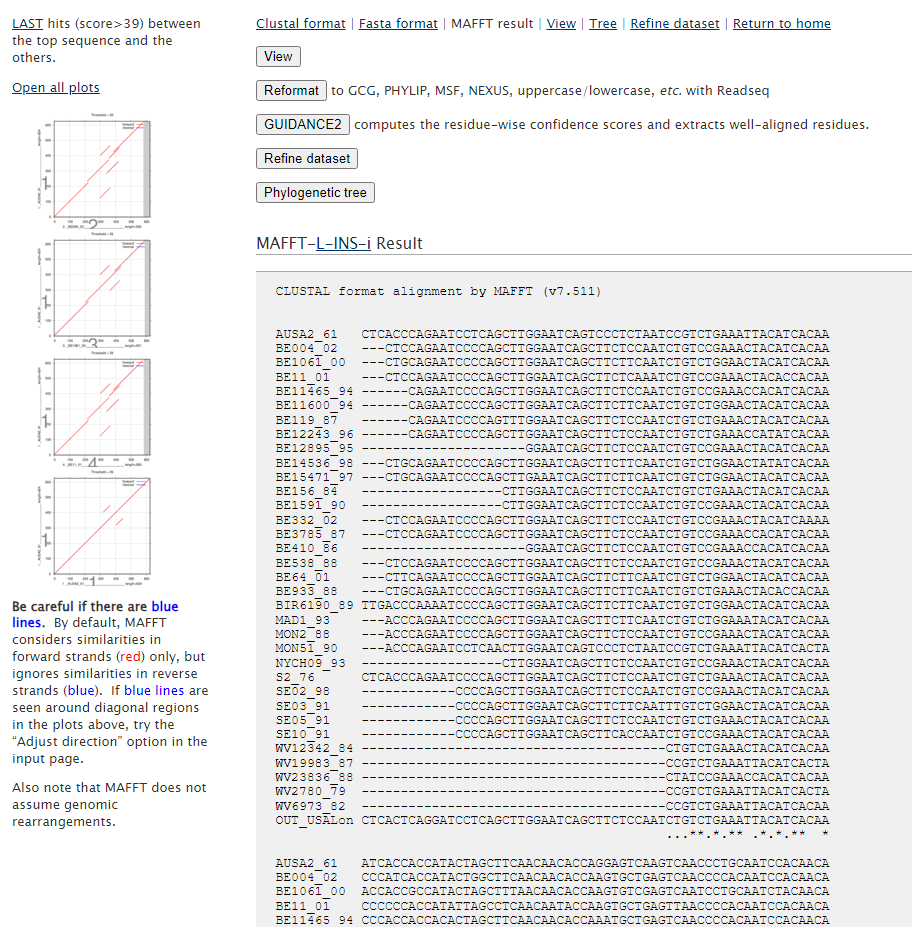
\includegraphics[width = \linewidth]{figs/mafft-result.png}
\caption{Resultado del alineamiento del fichero HRSV-A. La parte de la izquierda muestra unos gráficos de similitud. Debería estar todo en rojo, ya que si hay alguna línea en azul, eso indicaría que hay secuencias invertidas y que habría que reevaluar el alineamiento ajustando la direccionalidad.}
\label{fig:mafft-result}
\end{figure}

Para guardar el alineamiento, lo más cómodo es pulsar el botón de \texttt{Fasta format} en la parte superior. Este alineamiento lo podemos visualizar entonces en el programa de SeaView o en \href{http://phylemon.bioinfo.cipf.es/}{Phylemon}. \footnote{Tradicionalmente funcionaba bien en Google Chrome y daba error o no cargaba en otros navegadores. Ahora parece ser que es al revés; no carga usando Google Chrome, pero en Firefox funciona bien.} Este último tiene en el cluster programas de terceros para realizar alineamientos, árboles filogenéticos, test evolutivos y pipelines para combinarlos, pero también otras utilidades exclusivas. Dentro de las utilidades de alineamientos, hay tres programas: ConcatenAl permite concatenar los alineamientos, CDS-ProtAl sirve para traducir proteínas desde las secuencias codificantes, y TrimAl permite eliminar partes de la secuencia que están alineadas de forma dudosa o que tienen gaps. Nosotros vamos a utilizar CDS-ProtAl, donde podemos pegar una secuencia o subirla. Al subir un archivo, hay que seleccionarlo y decir el tipo de archivo que es (secuencia alineada, sin alinar, árbol, etc). Los parámetros que se pueden seleccionar son mantener o no los gaps y traducir la secuencia sin alinearla. También pide el código genético para poder traducir las proteínas. En nuestro caso del virus respiratorio sincitial humano, utilizaremos el código genético estándar. Una vez terminado el trabajo, nos podemos descargar los ficheros resultantes pulsando sobre el nombre o haciendo click derecho y "guardar enlace como". Aunque el formato sea out\_ali, se puede cambiar manualmente a fasta y visualizar con SeaView. 

Hay algunos casos en los que las regiones no alineadas pueden producir mucho ruido filogenético. Para eso, existen programas que permiten seleccionar bloques de secuencia conservada, como Gblocks o TrimAl. Desde Phylemon, se puede redirigir el resultado obtenido con CDS-ProtAl directamente a TrimAl (y otras herramientas) mediante un desplegable, facilitando así el trabajo y evitando tener que descargar los archivos intermedios y temporales. Antes de lanzar el trabajo con TrimAl, permite seleccionar la eliminación de secuencias de baja similitud o calidad antes de quitar las posiciones. Hay varios métodos para quitar los gaps: "no gaps" quita todas las posiciones que tengan un gap,"no all gaps" quita las posiciones que sólo sean gaps y no tengan ninguna secuencia, y "gappyout" quita las posiciones que tienen más gaps de lo esperado. 

Desde SeaView se puede también traducir una secuencia a proteínas mediante Props y el check de "ver como proteínas". En "File" se puede guardar el archivo. En algunos casos, algunas posiciones son muy variables (por ejemplo, las terceras posiciones de los genes mitocondriales, que tienen tantos cambios superimpuestos que no aportan información filogenética), por lo que es mejor eliminar las posiciones antes de realizar los análisis. En SeaView, esto se puede hacer en Sites y Create Set. A continuación se puede seleccionar aquellas posiciones que se quieren. Por ejemplo, para eliminar las terceras posiciones, habría que utilizar la opción que selecciona la primera y segunda posición. Para guardar esta selección, en File hay una opción de Save selection.
\section{Máxima parsimonia y visualización de árboles}
El objetivo de esta práctica es obtener árboles filogenéticos utilizando la máxima parsimonia utilizando un alineamiento de secuencias de ADN múltiple y visualizar los árboles con un visualizador gráfico. Los pasos para hacer esto en el programa de Mega son:
\begin{enumerate}
\item Abrir el archivo en File > Open a File/Session > Analyze. Selecciona el tipo de datos de acuerdo a su naturaleza, es decir, si se trata de nucleótidos, proteínas, si es codificante o no codificante, etc.
\item Construye el árbol en Phylogeny > Construct/Test Maximum Parsimony Tree(s). Hay varios campos con el borde resaltado que se pueden modificar:
\begin{itemize}
\item Test of Phylogeny: Sólo podemos hacer una búsqueda del árbol de máxima parsimonia, o también podemos hacer un análisis bootstrap. Si hacemos bootstrap, deberíamos hacer 1000 réplicas bootstrap, pero, dadas las limitaciones de tiempo, haremos 100 réplicas para este ejercicio.
\item Substitution Type: nucleótido o aminoácido si la secuencia de nucleótidos se ha marcado como codificante. Seleccionar aminoácidos aquí tendría el mismo efecto que eliminar la tercera posición de los análisis. 
\item Gaps/Missing Data Treatment: utiliza todos los sitios
\item Select Codon Positions: Prueba con varios árboles utilizando todas las posiciones, solo la primera y segunda posición, o solo la tercera posición.
\item MP Search Method: Tree-Bisection-Reconnection (TBR)
\item No. of initial trees (random addition): 10
\item MP Search level: 1
\item Max No. of trees to retain: 100
\item Compute (OK)
\end{itemize}
\item El árbol aparece en una nueva ventana. Si es necesario, se puede volver a enraizar en Subtree > Root.
\item Guardar el árbol desde File > Export Current Tree (Newick). Esto abre una ventana que se debe guardar pulsando en el botón del disquete o copiando y pegando en un documento de texto. El árbol se puede abrir y visualizar en un visualizador gráfico de árboles filogenéticos, como FigTree.
\end{enumerate}

El formato Newick utiliza los paréntesis para mostrar la jerarquía de los taxones en un árbol filogenético. También puede incluir las longitudes de las ramas o los valores de soporte del bootstrap. En ese caso, se utilizan los dos puntos con los taxones o con la relación (el paréntesis) respectivamente. 

FigTree está diseñado como visor gráfico de árboles filogenéticos y como programa para producir figuras listas para su publicación. Para visualizar el árbol con FigTree se realiza de la siguiente forma:
\begin{enumerate}
\item Abre el archivo del árbol (formato Newick o Nexus) en FigTree. Si el árbol está anotado (por ejemplo con valores adicionales en ramas/nodos), aparecerá una ventana solicitando un nombre específico para las anotaciones que el árbol tiene asociadas a sus nodos. En nuestro caso, se trata de los valores de soporte bootstrap, por lo que les daremos un nombre (por ejemplo, soporte).
\item Explora las opciones de enraizado, opciones de visualización y de ramas/nodos. Las distintas opciones se pueden seleccionar utilizando los paneles superiores o izquierdos. 
\end{enumerate}

Se puede cambiar el tamaño de la letra de los taxones desde Tip Labels > Font Size. También se puede enraizar un árbol desde FigTree, pulsando en una rama y en el botón de Reroot. Se pueden ordenar los nodos de forma ascendente o descendente desde Trees > Order nodes > Ordering y colorear las ramas en función de su valor de soporte. 

\begin{figure}[htbp]
\centering
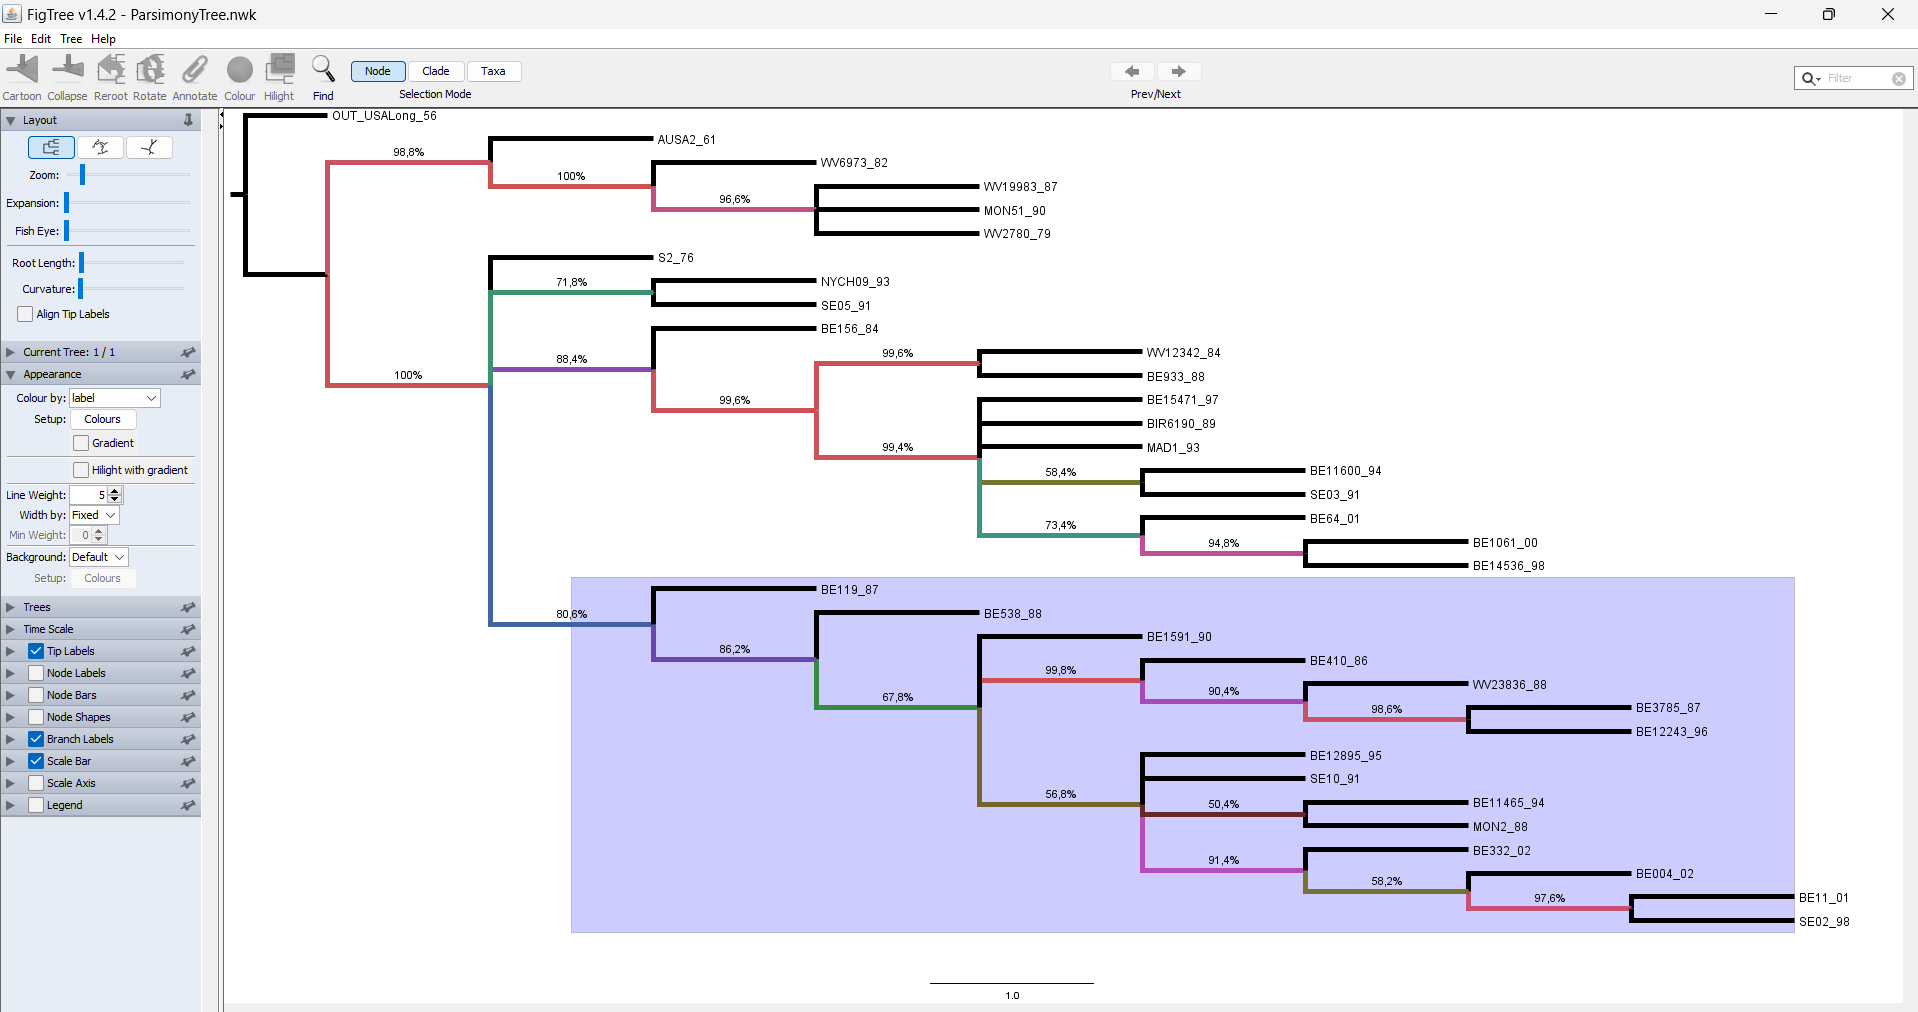
\includegraphics[width = \linewidth]{figs/figtree.png}
\end{figure}

Una de las plataformas para hacer árboles utilizando la máxima parsimonia es \href{https://www.lillo.org.ar/phylogeny/tnt/}{TNT}. El problema es que, pese a ser muy potente, es muy complicado de utilizar.
\section{Modelos de evolución}
El objetivo de esta práctica está en seleccionar el mejor modelo de sustitución para distintos tipos de datos: nucleótidos y aminoácidos. Para seleccionar el \textbf{mejor modelo de sustitución de nucleótidos} desde el servidor de IQ-Tree se deben realizar los siguientes pasos:
\begin{enumerate}
\item Ve al \href{http://iqtree.cibiv.univie.ac.at/}{servidor de la web de IQ-Tree}.
\item Cambia a la pestaña de Selección de Modelos.
\item Carga el fichero del alineamiento de nucleótidos.
\item Selecciona el tipo de secuencia (en este caso ADN) o déjalo como detección automática.
\item Cambia los criterios de selección a AIC para este ejercicio.
\item No cambies ninguna otra opción.
\item Opcional: deja un correo electrónico para poder obtener los resultados directamente.
\item Pulsa a submit job.
\item Una vez terminado, comprueba los resultados en la ventada de Full Results. Descarga los resultados y examina los distintos archivos en editores de texto plano.
\end{enumerate}

Para seleccionar el \textbf{mejor modelo de sustitución de aminoácidos} desde el servidor de IQ-Tree se deben realizar los siguientes pasos:
\begin{enumerate}
\item Ve al \href{http://iqtree.cibiv.univie.ac.at/}{servidor de la web de IQ-Tree}.
\item Cambia a la pestaña de Selección de Modelos.
\item Carga el fichero del alineamiento de nucleótidos.
\item Selecciona el tipo de secuencia DNA -> AA, carga el alineamiento de aminoácidos y selecciona Protein o déjalo como detección automática.
\item Elige el código genético apropiado (en este caso, estándar o universal).
\item Cambia los criterios de selección a AIC para este ejercicio.
\item No cambies ninguna otra opción.
\item Opcional: deja un correo electrónico para poder obtener los resultados directamente.
\item Pulsa a submit job.
\item Una vez terminado, comprueba los resultados en la ventada de Full Results. Descarga los resultados y examina los distintos archivos en editores de texto plano.
\end{enumerate}

Si sabemos que nuestros datos son ADN o aminoácidos, es mejor indicar en IQ-Tree el tipo de secuencia que no dejar que lo detecte de forma automática. Esto se debe a que las letras de los nucleótidos también se utilizan en los aminoácidos, y a la hora de analizar SNPs puede detectar algo erróneo. 

El documento descargado .iqtree muestra lo mismo que lo que se vería en la pestaña de Full Result. Los modelos aparecen por orden descendente de ajuste (el primero que aparece es el que mejor se ajusta, que suele ser el más complejo; el último es el que menos se ajusta, y suele ser el más sencillo). También muestra los parámetros de tasas de sustitución y frecuencia

\end{document}
